\documentclass[../main.tex]{subfiles}

\begin{document}


\section{Random Matrix Theory}
A lot of physical systems -- e.g. systems with glassy dynamics -- can often be modeled using graphs.
This makes graph theory an integral part of physics itself and it has been studied extensively.
In this exercise we will look at such systems that additionally contain disorder. 
Every regular graph can be expressed as an adjacency matrix which can be used to analyze the system.
\par

\subsection{Analysis by Direct Diagonalization}

\subsubsection{Sparse Random Matrix}
In the first step of our analysis we use well known techniques to establish a baseline for our methodology.
The method we use is called Direct Diagonalization and it obtains the spectrum of the system by using numeric Exact Diagonalization (ED).
\par 

\begin{figure}[htpb]
    \centering
    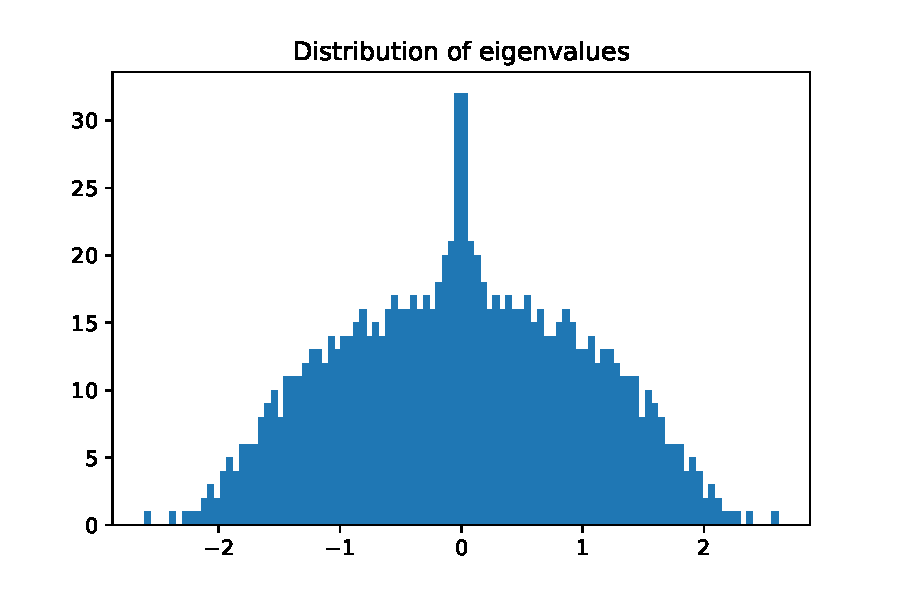
\includegraphics[width=0.8\textwidth]{../figures/2_1_1_spectrum_sparse.pdf}
    \caption{Spectrum of a RRG of size \num{2^{10}} with connectivity \num{3} averaged over 10 different instances.}
    \label{fig:spectrum_sparse}
\end{figure}

In a first analysis step we generate \num{10} different Random Regular Graphs (RRG) and calculate their spectrum vie ED and average their spectrum.
In Figure \ref{fig:spectrum_sparse} you can see the average spectrum of the RRGs of size $N = 2^{10}$ with connectivity 3.



\subsection{Analysis by Cavity Method}


\ifSubfilesClassLoaded{
	% if it's compiled alone
}{
	% if it's compiled in the main file
    \newpage
}
\end{document}
    
\end{document} 
